% ==============================================================================
% PRESENTACIÓN AVANCE 2 — ANÁLISIS DE DATOS E INFERENCIA ESTADÍSTICA (UDD)
% Modelado Estadístico Inferencial y Predictivo de Material Particulado
% (MP10 y PM2.5) en la Estación Kingston College (2009–2026)
%
% Integrantes: Javier Benavides Ortega & Cristóbal Montoya Toledo
% Docente:     Prof. Danilo Gómez Correa
% Duración:    15–20 minutos (21 diapositivas)
% ==============================================================================

\documentclass[aspectratio=169, 9pt]{beamer}

% --- Codificación, Idioma y Fuentes ---
\usepackage[utf8]{inputenc}
\usepackage[T1]{fontenc}
\usepackage[spanish,es-nodecimaldot]{babel}
\usepackage{lmodern}
\usepackage{microtype}

% --- Matemáticas, Tablas y Gráficos ---
\usepackage{amsmath, amssymb, amsfonts, mathtools}
\usepackage{booktabs}
\usepackage{array}
\usepackage{graphicx}
\usepackage{xcolor}

% --- Ruta de Imágenes ---
\graphicspath{{../../assets/figuras/}{./}}

% --- Tema Beamer Limpio (Estilo Clases Prof. Danilo Gómez) ---
\usetheme{default}
\usefonttheme{professionalfonts}

% --- Paleta de Colores Académica y Suave ---
\definecolor{UddNavy}{RGB}{20, 50, 110}      % Azul universitario principal
\definecolor{UddBlue}{RGB}{35, 85, 175}      % Azul para títulos y acentos
\definecolor{NaturalAmber}{RGB}{185, 85, 10} % Ámbar para hipótesis en lenguaje natural
\definecolor{MathGreen}{RGB}{20, 115, 55}    % Verde para formulación matemática y decisiones
\definecolor{DarkGray}{RGB}{40, 45, 55}      % Texto general
\definecolor{LightBg}{RGB}{246, 248, 252}    % Fondo suave para bloques estándar
\definecolor{LightAmber}{RGB}{255, 248, 240} % Fondo suave para bloques de lenguaje natural
\definecolor{LightGreen}{RGB}{242, 250, 244} % Fondo suave para bloques matemáticos

\setbeamercolor{background canvas}{bg=white}
\setbeamercolor{normal text}{fg=DarkGray}
\setbeamercolor{structure}{fg=UddBlue}
\setbeamercolor{title}{fg=UddNavy}
\setbeamercolor{frametitle}{fg=UddNavy, bg=white}
\setbeamercolor{framesubtitle}{fg=UddBlue!80!black}

% Estilo de bloques NATIVOS de Beamer
\setbeamercolor{block title}{bg=UddNavy, fg=white}
\setbeamercolor{block body}{bg=LightBg, fg=DarkGray}

\setbeamercolor{block title alerted}{bg=NaturalAmber, fg=white}
\setbeamercolor{block body alerted}{bg=LightAmber, fg=DarkGray}

\setbeamercolor{block title example}{bg=MathGreen, fg=white}
\setbeamercolor{block body example}{bg=LightGreen, fg=DarkGray}

% Márgenes laterales amplios y espaciado matemático compacto (evita desbordes inferiores)
\setbeamersize{text margin left=7mm, text margin right=7mm}
\setlength{\abovedisplayskip}{2pt}
\setlength{\belowdisplayskip}{2pt}
\setlength{\abovedisplayshortskip}{1pt}
\setlength{\belowdisplayshortskip}{1pt}

% Limpieza de íconos de navegación
\setbeamertemplate{navigation symbols}{}
\setbeamertemplate{itemize items}[circle]
\setbeamertemplate{enumerate items}[default]

% Frametitle compacto (ahorra altura vertical en todas las diapositivas)
\makeatletter
\setbeamertemplate{frametitle}{
  \vspace{0.10cm}
  {\normalsize\bfseries\color{UddNavy}\insertframetitle}\par
  \ifx\insertframesubtitle\@empty\else
    \vspace{0.02cm}
    {\scriptsize\color{UddBlue}\insertframesubtitle}\par
  \fi
  \vspace{-0.18cm}
  {\color{UddNavy!20!white}\hrulefill}
  \vspace{0.02cm}
}
\makeatother

% Pie de página minimalista (1 sola línea limpia)
\setbeamertemplate{footline}{
  \leavevmode%
  \hbox{%
  \begin{beamercolorbox}[wd=.333\paperwidth,ht=2.0ex,dp=0.6ex,left,leftskip=7mm]{author in head/foot}%
    \tiny\color{gray}\textbf{J. Benavides \& C. Montoya} (UDD)
  \end{beamercolorbox}%
  \begin{beamercolorbox}[wd=.333\paperwidth,ht=2.0ex,dp=0.6ex,center]{title in head/foot}%
    \tiny\color{gray}Avance 2: Modelado Estadístico e Inferencia ($MP_{10} \to PM_{2.5}$)
  \end{beamercolorbox}%
  \begin{beamercolorbox}[wd=.333\paperwidth,ht=2.0ex,dp=0.6ex,right,rightskip=7mm]{date in head/foot}%
    \tiny\color{gray}Prof. Danilo Gómez Correa \quad $|$ \quad \insertframenumber{} / \inserttotalframenumber
  \end{beamercolorbox}}%
  \vskip0pt%
}

% Metadatos del Documento
\title{Modelado Estadístico Inferencial y Predictivo de Material Particulado ($MP_{10}$ y $PM_{2.5}$)}
\subtitle{Avance 2: Modelamiento EMCO, Diagnóstico de Supuestos e Inferencia en Kingston College (2009–2026)}
\author{\textbf{Javier Benavides Ortega} \and \textbf{Cristóbal Montoya Toledo}}
\institute{Facultad de Ingeniería — Universidad del Desarrollo \\ Curso: Análisis de Datos e Inferencia Estadística \\ \textbf{Profesor Guía:} Danilo Gómez Correa}
\date{Noviembre 2026}

\begin{document}

% ==============================================================================
% DIAPOSITIVA 1: PORTADA LIMPIA
% ==============================================================================
\begin{frame}[plain]
  \vspace{0.4cm}
  \begin{center}
    {\scriptsize\bfseries\color{UddBlue} UNIVERSIDAD DEL DESARROLLO $\bullet$ FACULTAD DE INGENIERÍA}\\[0.12cm]
    {\scriptsize\color{DarkGray} ANÁLISIS DE DATOS E INFERENCIA ESTADÍSTICA $\bullet$ AVANCE 2}\\[0.35cm]
    
    {\Large\bfseries\color{UddNavy} Modelado Estadístico Inferencial y Predictivo\\de Material Particulado ($MP_{10}$ y $PM_{2.5}$)}\\[0.2cm]
    {\small\color{UddBlue} Estación Kingston College, Red SINCA Concepción (2009–2026)}\\[0.35cm]
    
    {\color{UddNavy!25!white}\rule{0.65\textwidth}{0.8pt}}\\[0.35cm]
    
    {\small\textbf{Integrantes:} Javier Benavides Ortega \quad \& \quad Cristóbal Montoya Toledo}\\[0.12cm]
    {\small\textbf{Profesor Guía:} Danilo Gómez Correa}\\[0.25cm]
    
    \begin{beamercolorbox}[wd=0.88\textwidth, rounded=true, center, sep=4pt]{block body}
      \scriptsize\color{DarkGray}
      \textbf{Énfasis Metodológico Aplicado:} En todas las pruebas estadísticas realizadas en el estudio se explicita su \textbf{Hipótesis Nula ($H_0$) y Alternativa ($H_1$) en Formato Texto Natural} (cajas ámbar) y en \textbf{Formato Matemático} (cajas verdes).
    \end{beamercolorbox}
    
    \vspace{0.15cm}
    {\scriptsize\color{gray} Duración Estimada: 15–20 minutos Concepción, Chile}
  \end{center}
\end{frame}

% ==============================================================================
% DIAPOSITIVA 2: CONTEXTO FÍSICO, SANITARIO Y VACÍO DE INVESTIGACIÓN
% ==============================================================================
\begin{frame}{1. Contextualización Física, Literatura y Magnitud del Corpus}
\framesubtitle{Fenómeno de co-emisión y representatividad de la estación Kingston College}

\begin{columns}[T]
  \begin{column}{0.48\textwidth}
    \begin{block}{\footnotesize Fundamento Físico: $PM_{2.5} \subseteq MP_{10}$}
      \scriptsize
      \begin{itemize}\setlength{\itemsep}{2.5pt}
        \item La fracción fina respirable ($PM_{2.5} \le 2.5\,\mu\text{m}$) está \textbf{físicamente contenida} dentro del material particulado grueso ($MP_{10} \le 10\,\mu\text{m}$).
        \item \textbf{Cereceda-Balic et al. (2020):} En invierno del centro-sur de Chile, el $PM_{2.5}$ constituye entre el \textbf{65\% y 80\%} del $MP_{10}$ debido a la combustión residencial de leña.
        \item \textbf{Saide et al. (2016):} Inversiones térmicas de subsidencia en la cuenca de Concepción provocan estancamiento atmosférico multidiario.
        \item \textbf{Gramsch et al. (2021):} La caída del tráfico laboral en pandemia no disminuyó el $PM_{2.5}$ invernal por el peso de la calefacción domiciliaria.
      \end{itemize}
    \end{block}
  \end{column}

  \begin{column}{0.48\textwidth}
    \begin{alertblock}{\footnotesize Vacío de Conocimiento Identificado (\textit{Gap})}
      \scriptsize
      Inexistencia de modelos inferenciales y multivariables continuos (2009–2026) a escala diaria en \textbf{Kingston College} que integren simultáneamente \textbf{gases trazadores ($CO, NO_2, O_3$)} y factores estacionales bajo auditoría de supuestos del EMCO.
    \end{alertblock}

    \begin{block}{\footnotesize Magnitud del Corpus de Datos (SINCA)}
      \scriptsize
      \begin{itemize}\setlength{\itemsep}{2pt}
        \item \textbf{Total registros brutos:} $893.398$ filas (16 archivos CSV).
        \item \textbf{Cobertura temporal:} 17,2 años (Agosto 2009 – Octubre 2026).
        \item \textbf{Días pareados limpios:} $n = \mathbf{3.280}$ ($n = \mathbf{3.185}$ con gases).
      \end{itemize}
    \end{block}
  \end{column}
\end{columns}
\end{frame}

% ==============================================================================
% DIAPOSITIVA 3: PREGUNTA DE INVESTIGACIÓN E HIPÓTESIS CENTRAL (DUAL)
% ==============================================================================
\begin{frame}{1.2 y 1.3. Pregunta de Investigación e Hipótesis Central del Estudio}
\framesubtitle{Formulación Dual: Texto Natural y Notación Matemática}

\begin{beamercolorbox}[wd=\textwidth, rounded=true, sep=3pt]{block body}
  \scriptsize\textbf{Pregunta de Investigación:} ¿En qué medida los niveles diarios de $MP_{10}$ y gases de combustión predicen la concentración de $PM_{2.5}$ en Kingston College (2009–2026), y cómo varía según la estación del año y el tipo de día?
\end{beamercolorbox}

\vspace{0.06cm}
\begin{columns}[T]
  \begin{column}{0.48\textwidth}
    \begin{alertblock}{\footnotesize Hipótesis Central — Formato Texto Natural}
      \scriptsize
      \begin{itemize}\setlength{\itemsep}{2pt}
        \item \textbf{$H_0$ (\textit{Status Quo}):} No existe una relación lineal ni monótona estadísticamente significativa entre los niveles diarios de $MP_{10}$ y $PM_{2.5}$ en Kingston College; las variaciones de $MP_{10}$ y gases no tienen capacidad predictiva real sobre el $PM_{2.5}$.
        \item \textbf{$H_1$ (Efecto Investigado):} Existe una asociación positiva estadísticamente significativa donde mayores concentraciones diarias de $MP_{10}$ (y del trazador de leña $CO$ en invierno) predicen incrementos directos de $PM_{2.5}$.
      \end{itemize}
    \end{alertblock}
  \end{column}

  \begin{column}{0.48\textwidth}
    \begin{exampleblock}{\footnotesize Hipótesis Central — Formato Matemático}
      \scriptsize
      Modelo poblacional $PM_{2.5, i} = \beta_0 + \beta_1 MP_{10, i} + \sum_{j=2}^p \beta_j X_{ij} + \epsilon_i$:
      $$H_0: \beta_1 = 0 \;\wedge\; \rho = 0 \qquad \text{vs.} \qquad H_1: \beta_1 > 0 \;\wedge\; \rho > 0$$
      \begin{itemize}\setlength{\itemsep}{1.5pt}
        \item \textbf{Error Tipo I ($\alpha$):} $\alpha = \Pr(\text{Rechazar } H_0 \mid H_0 \text{ cierta}) = 0.05$.
        \item \textbf{Error Tipo II ($\beta$):} $\beta = \Pr(\text{No rechazar } H_0 \mid H_0 \text{ falsa})$.
        \item \textbf{Escala Valor-$p$ (\alpha = 0.05):}
        \begin{itemize}\scriptsize
          \item $(v-p) < 0.01$: \textbf{Evidencia muy fuerte} contra $H_0$ (Rechazar $H_0$).
          \item $(v-p) > 0.10$: \textbf{No se rechaza $H_0$} (Evidencia insuficiente).
        \end{itemize}
      \end{itemize}
    \end{exampleblock}
  \end{column}
\end{columns}
\end{frame}

% ==============================================================================
% DIAPOSITIVA 4: ETAPA 1 Y 2 DEL EDA — DESCRIPTIVOS Y CODIFICACIÓN DUMMY
% ==============================================================================
\begin{frame}{2. Etapas 1 y 2 del EDA: Análisis Descriptivo y Codificación Dummy}
\framesubtitle{Caracterización univariada, Regla de Sturges y prevención de colinealidad exacta}

\begin{columns}[T]
  \begin{column}{0.48\textwidth}
    \begin{block}{\footnotesize Estadísticos Descriptivos (Etapa 1)}
      \renewcommand{\arraystretch}{0.96}
      \resizebox{\linewidth}{!}{
        \begin{tabular}{llrr}
          \toprule
          \textbf{Medida} & \textbf{Símbolo} & \textbf{$MP_{10}$ ($\mu\text{g/m}^3$)} & \textbf{$PM_{2.5}$ ($\mu\text{g/m}^3$)} \\
          \midrule
          Muestras válidas & $n$ & $4.812$ & $3.312$ \\
          Mínimo / Máximo & $z_{\min} / z_{\max}$ & $3.00 / 173.00$ & $1.00 / 121.00$ \\
          Primer Cuartil & $Q_1$ & $18.00$ & $7.00$ \\
          \textbf{Mediana} & $z_m$ & $\mathbf{26.00}$ & $\mathbf{11.00}$ \\
          \textbf{Media} & $\bar{z}$ & $\mathbf{28.91}$ & $\mathbf{14.19}$ \\
          Tercer Cuartil & $Q_3$ & $36.00$ & $19.00$ \\
          Rango Intercuartil & $RIC$ & $18.00$ & $12.00$ \\
          Desv. Estándar & $s$ & $15.83$ & $10.83$ \\
          Coef. Variación & $CV$ & $54.76\%$ & $\mathbf{76.31\%}$ \\
          \textbf{Asimetría} & $k_s$ & $\mathbf{+1.84}$ (Sesgo $+$) & $\mathbf{+2.05}$ (Sesgo $+$) \\
          \bottomrule
        \end{tabular}
      }
    \end{block}
    {\tiny \textbf{Regla de Sturges ($PM_{2.5}$):} $k = 1 + 3.322\log_{10}(3312) = 13$ int. ($\text{ancho} = 9.45\,\mu\text{g/m}^3$). El \textbf{89.9\%} se acumula en los primeros 3 intervalos.}
  \end{column}

  \begin{column}{0.48\textwidth}
    \begin{block}{\footnotesize Codificación Dummy $k-1$ (Sección 3.6)}
      \scriptsize
      Para evitar la \textbf{trampa de variables ficticias} (violación del Supuesto 2 de Rango Completo por colinealidad con el intercepto $\beta_0$):
      \begin{itemize}\setlength{\itemsep}{2pt}
        \item \textbf{Estación del Año ($k=4 \to 3$ Dummies, Base = Verano):}
        $$D_{\text{Oto}}, D_{\text{Inv}}, D_{\text{Pri}} \in \{0, 1\}$$
        Cuando las tres son $0$, $\beta_0$ refleja el nivel basal de \textbf{Verano}.
        \item \textbf{Tipo de Día ($k=2 \to 1$ Binaria, Base = Laboral):}
        $$\text{Es\_FDS} = 1 \text{ (Sáb--Dom)}, \quad 0 \text{ (Lun--Vie)}$$
      \end{itemize}
    \end{block}
    
    \begin{beamercolorbox}[wd=\textwidth, rounded=true, sep=2.5pt]{block body}
      \tiny\textbf{Filtro Físico:} Se descartaron 32 días con $PM_{2.5} > MP_{10}$ por descalibración instrumental beta (SMA, 2024), evitando sesgo de atenuación.
    \end{beamercolorbox}
  \end{column}
\end{columns}
\end{frame}

% ==============================================================================
% DIAPOSITIVA 5: ETAPA 3 DEL EDA — NULOS (MCAR vs MAR)
% ==============================================================================
\begin{frame}{2.1. Etapa 3 del EDA: Tratamiento de Datos Nulos (MCAR vs. MAR)}
\framesubtitle{Justificación metodológica para no imputar con la media en series ambientales}

\begin{columns}[T]
  \begin{column}{0.48\textwidth}
    \centering
    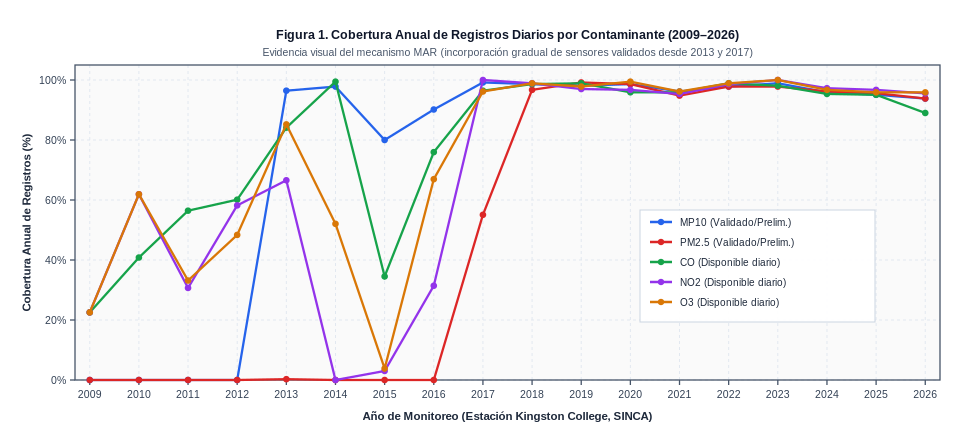
\includegraphics[width=\linewidth, height=0.52\textheight, keepaspectratio]{fig1_completitud_temporal.png}
    \vspace{0.03cm}
    {\tiny Cobertura anual de contaminantes SINCA en Kingston College (2009–2026).}
  \end{column}

  \begin{column}{0.48\textwidth}
    \begin{block}{\footnotesize Diagnóstico de Mecanismos (Fig. 1)}
      \scriptsize
      \begin{itemize}\setlength{\itemsep}{2pt}
        \item \textbf{MAR (\textit{Missing At Random}):} La ausencia de $PM_{2.5}$ antes de 2013/2017 depende del año de instalación del sensor en Kingston College.
        \item \textbf{MCAR (\textit{Missing Completely At Random}):} Cortes eléctricos o mantención programada de filtros ($\approx 10\%$).
      \end{itemize}
    \end{block}

    \begin{alertblock}{\footnotesize ¿Por qué NO imputar con la Media $\bar{z}$?}
      \scriptsize
      Fundamentación estadística:
      \begin{enumerate}\scriptsize\setlength{\itemsep}{1pt}
        \item \textbf{Subestima la varianza} y aplana las preemergencias invernales.
        \item \textbf{Distorsiona la covarianza} y correlación entre contaminantes al inyectar constantes repetidas.
        \item \textbf{Decisión:} Trabajar con \textbf{Casos Completos} ($n = 3.280$ días validados).
      \end{enumerate}
    \end{alertblock}
  \end{column}
\end{columns}
\end{frame}

% ==============================================================================
% DIAPOSITIVA 6: ETAPA 4 DEL EDA (2.2) — ATÍPICOS, GRUBBS Y WINSORIZACIÓN
% ==============================================================================
\begin{frame}{2.2. Etapa 4 del EDA: Valores Atípicos, Grubbs y Winsorización}
\framesubtitle{Test N° 1: Contraste Formal de Valores Extremos de Grubbs}

\begin{columns}[T]
  \begin{column}{0.46\textwidth}
    \centering
    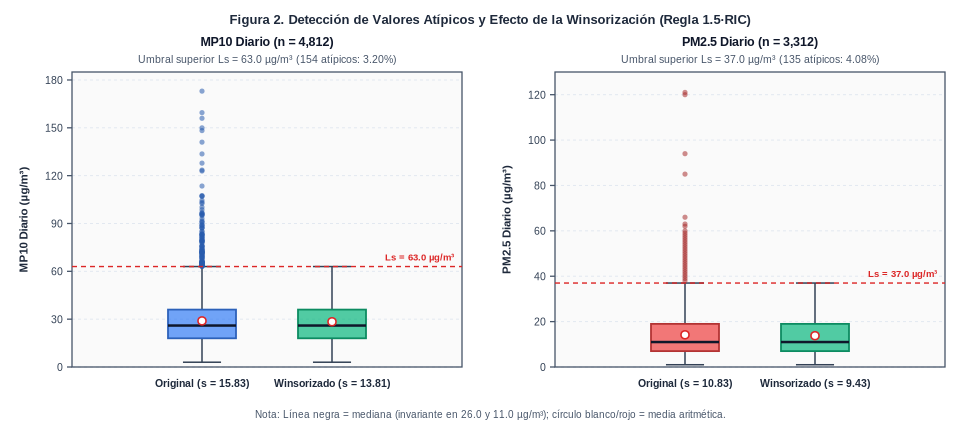
\includegraphics[width=\linewidth, height=0.42\textheight, keepaspectratio]{fig2_outliers_winsorizacion.png}
    \vspace{0.03cm}
    \begin{beamercolorbox}[wd=\linewidth, rounded=true, sep=2pt]{block body}
      \tiny\textbf{Efecto Winsorización ($L_s = Q_3 + 1.5\cdot RIC$):} En $PM_{2.5}$ ($L_s=37\,\mu\text{g/m}^3$, $135$ atípicos), $s$ cae $-12.9\%$ ($10.83 \to 9.43$), pero la \textbf{mediana no cambia} ($11.0\,\mu\text{g/m}^3$, $\text{MAD}=5.0$).
    \end{beamercolorbox}
  \end{column}

  \begin{column}{0.50\textwidth}
    \begin{alertblock}{\footnotesize Test 1 (Grubbs) — Hipótesis en Texto Natural}
      \scriptsize
      \begin{itemize}\setlength{\itemsep}{1pt}
        \item \textbf{$H_0$:} No existen valores atípicos extremos en la serie diaria de particulado; el máximo observado es compatible con la dispersión aleatoria normal.
        \item \textbf{$H_1$:} Existe al menos un valor atípico extremo en la serie diaria cuya magnitud se aleja significativamente del promedio muestral.
      \end{itemize}
    \end{alertblock}

    \begin{exampleblock}{\footnotesize Test 1 (Grubbs) — Hipótesis en Formato Matemático}
      \scriptsize
      \begin{itemize}\setlength{\itemsep}{1pt}
        \item \textbf{Hipótesis:} $H_0: \text{Sin outliers en } \{X_i\}_{i=1}^N \quad \text{vs.} \quad H_1: \max_i |X_i - \bar{X}|/S \text{ es extremo}$.
        \item \textbf{Estadístico y Criterio ($\alpha=0.05$):} $G = \frac{\max_i |X_i - \bar{X}|}{S} > G_{\text{crit}}(0.05, N) \approx 4.30$.
        \item \textbf{Resultados:} $MP_{10}: G = \mathbf{9.10} > 4.39$ ($p<.001$); $PM_{2.5}: G = \mathbf{9.87} > 4.30$ ($p<.001$).
        \item \textbf{Decisión:} \textbf{Se rechaza $H_0$}. Son \textbf{atípicos naturales reales} (preemergencias de invierno); se conservan para modelar las crisis sanitarias.
      \end{itemize}
    \end{exampleblock}
  \end{column}
\end{columns}
\end{frame}

% ==============================================================================
% DIAPOSITIVA 7: ETAPA 5.1 — PRUEBAS DE BONDAD DE AJUSTE (NORMALIDAD)
% ==============================================================================
\begin{frame}{3. Etapa 5.1: Pruebas de Bondad de Ajuste y Lognormalidad}
\framesubtitle{Tests N° 2 y 3: Kolmogórov-Smirnov ($D$) y Anderson-Darling ($A^{2*}$)}

\begin{columns}[T]
  \begin{column}{0.46\textwidth}
    \centering
    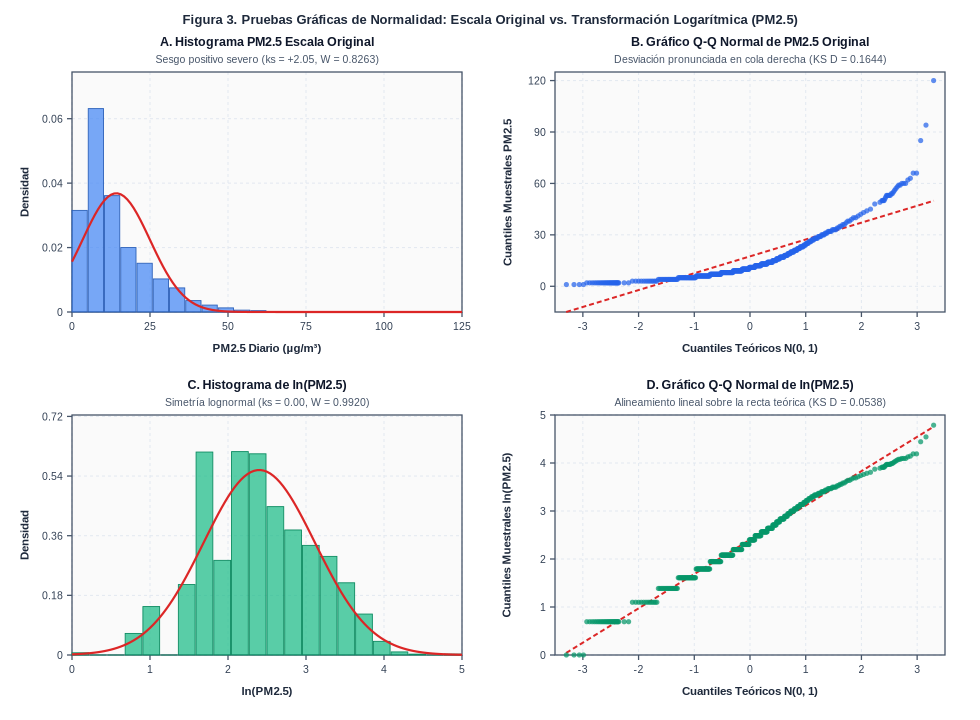
\includegraphics[width=\linewidth, height=0.45\textheight, keepaspectratio]{fig3_histograma_qq_normalidad.png}
    \vspace{0.02cm}
    {\tiny Con $\ln(PM_{2.5})$ la asimetría cae de $+2.05$ a $\mathbf{0.00}$ ($\bar{z}=z_m=2.40$) y $A^{2*}$ baja un $94\%$ ($151.16 \to 8.47$).}
  \end{column}

  \begin{column}{0.50\textwidth}
    \begin{alertblock}{\footnotesize Tests 2 y 3 (KS y AD) — Hipótesis en Texto Natural}
      \scriptsize
      \begin{itemize}\setlength{\itemsep}{1pt}
        \item \textbf{$H_0$:} Las concentraciones diarias de $MP_{10}$ y $PM_{2.5}$ provienen de una distribución Normal simétrica tanto en su centro (KS) como en sus colas (AD).
        \item \textbf{$H_1$:} Las concentraciones diarias no siguen una distribución Normal, presentando asimetría positiva y colas extremas pesadas.
      \end{itemize}
    \end{alertblock}

    \begin{exampleblock}{\footnotesize Tests 2 y 3 (KS y AD) — Hipótesis en Formato Matemático}
      \scriptsize
      \begin{itemize}\setlength{\itemsep}{1pt}
        \item \textbf{Hipótesis:} $H_0: F_X(x) = \Phi\left(\frac{x-\mu}{\sigma}\right) \;\;\forall x \quad \text{vs.} \quad H_1: F_X(x) \neq \Phi\left(\frac{x-\mu}{\sigma}\right)$.
        \item \textbf{Test 2 (KS):} $D = \max\{D^+, D^-\} = \mathbf{0.1644} > D_{0.05} = \frac{1.36}{\sqrt{n}} = 0.0236$ ($p < 0.001$).
        \item \textbf{Test 3 (AD):} $A^{2*} = \mathbf{151.16} \gg A^2_{\text{crit}}(0.05) = 0.787$ ($p < 0.001$).
        \item \textbf{Decisión:} \textbf{Se rechaza $H_0$} en escala original. El proceso físico es \textbf{Lognormal}, justificando métodos duales y el \textbf{Modelo 4 Log-Log}.
      \end{itemize}
    \end{exampleblock}
  \end{column}
\end{columns}
\end{frame}

% ==============================================================================
% DIAPOSITIVA 8: ETAPA 5.2 (PARTE A) — CORRELACIÓN BIVARIADA (PEARSON Y SPEARMAN)
% ==============================================================================
\begin{frame}{3.1. Etapa 5.2 (Parte A): Correlación Bivariada ($MP_{10}$ vs. $PM_{2.5}$)}
\framesubtitle{Tests N° 4 y 5: Correlación Lineal de Pearson ($r$) y Monótona de Spearman ($r_s$)}

\begin{columns}[T]
  \begin{column}{0.46\textwidth}
    \centering
    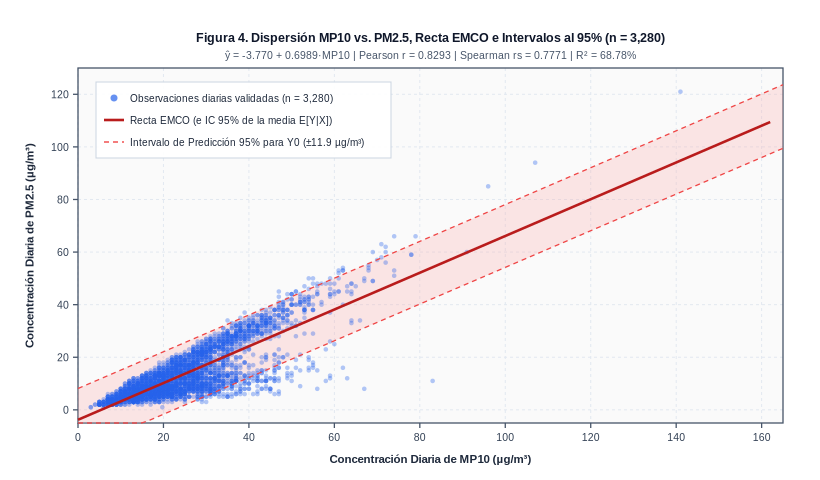
\includegraphics[width=\linewidth, height=0.45\textheight, keepaspectratio]{fig4_dispersion_mp10_pm25.png}
    \vspace{0.02cm}
    {\tiny Dispersión diaria validada ($n = 3.280$), recta EMCO $\hat{y} = -3.77 + 0.6989\,x$ y bandas al $95\%$.}
  \end{column}

  \begin{column}{0.50\textwidth}
    \begin{alertblock}{\footnotesize Tests 4 y 5 (Pearson y Spearman) — Texto Natural}
      \scriptsize
      \begin{itemize}\setlength{\itemsep}{1pt}
        \item \textbf{$H_0$:} No existe asociación lineal (Pearson) ni dependencia monótona por rangos (Spearman) entre los niveles diarios de $MP_{10}$ y $PM_{2.5}$.
        \item \textbf{$H_1$:} Existe una asociación positiva directa y significativa: días con mayor concentración de $MP_{10}$ presentan mayor concentración de $PM_{2.5}$.
      \end{itemize}
    \end{alertblock}

    \begin{exampleblock}{\footnotesize Tests 4 y 5 (Pearson y Spearman) — Formato Matemático}
      \scriptsize
      \begin{itemize}\setlength{\itemsep}{1.5pt}
        \item \textbf{Test 4 (Pearson):} $H_0: \rho = 0 \;\;\text{vs.}\;\; H_1: \rho > 0 \quad \Big|\quad t_c = \frac{r\sqrt{n-2}}{\sqrt{1-r^2}} \sim t_{(3278)}$.\\
        Resultado: $r = \mathbf{0.8293} \implies t_c = \mathbf{84.98} > 1.9607$ ($p < 10^{-16}$). \textbf{Rechaza $H_0$}.
        \item \textbf{Test 5 (Spearman):} $H_0: \rho_s = 0 \;\;\text{vs.}\;\; H_1: \rho_s > 0 \quad \Big|\quad z_s = r_s\sqrt{n-1} \sim \mathcal{N}(0,1)$.\\
        Resultado: $r_s = \mathbf{0.7771} \implies z_s = \mathbf{44.49} > 1.96$ ($p < 10^{-16}$). \textbf{Rechaza $H_0$}.
      \end{itemize}
    \end{exampleblock}
  \end{column}
\end{columns}
\end{frame}

% ==============================================================================
% DIAPOSITIVA 9: ETAPA 5.2 (PARTE B) — MATRIZ MULTIVARIADA CON GASES
% ==============================================================================
\begin{frame}{3.2. Etapa 5.2 (Parte B): Correlación Multivariada con Gases Trazadores}
\framesubtitle{Co-emisión con Monóxido de Carbono ($CO$), $NO_2$ y relación inversa con Ozono ($O_3$)}

\begin{columns}[T]
  \begin{column}{0.48\textwidth}
    \centering
    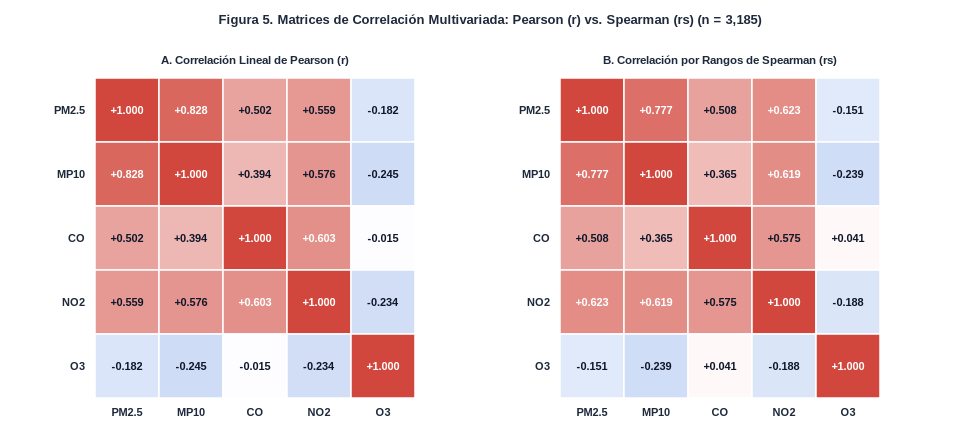
\includegraphics[width=\linewidth, height=0.46\textheight, keepaspectratio]{fig5_heatmap_correlaciones.png}
    \vspace{0.02cm}
    {\tiny Matrices de correlación de Pearson ($r$) y Spearman ($r_s$) sobre muestra común con gases ($n = 3.185$).}
  \end{column}

  \begin{column}{0.48\textwidth}
    \begin{block}{\footnotesize Interpretación Físico-Química de la Matriz (Fig. 5)}
      \scriptsize
      \begin{itemize}\setlength{\itemsep}{2.5pt}
        \item \textbf{Trazador de biomasa residencial ($CO$):} Presenta correlación positiva significativa con $PM_{2.5}$ ($r = \mathbf{+0.502}, r_s = \mathbf{+0.508}, p < 10^{-16}$), confirmando la emisión conjunta por combustión incompleta de leña.
        \item \textbf{Precursor urbano ($NO_2$):} Correlaciona positivamente con $PM_{2.5}$ ($r = +0.559$) y con $CO$ ($r = +0.603$), anticipando colinealidad moderada que será evaluada vía \textbf{VIF} en la regresión múltiple.
        \item \textbf{Comportamiento opuesto del Ozono ($O_3$):} Exhibe asociación negativa con $PM_{2.5}$ ($r = \mathbf{-0.182}, r_s = -0.151$), ya que el $O_3$ es un gas secundario fotoquímico de máxima radiación estival (verano), opuesto al invierno.
      \end{itemize}
    \end{block}
  \end{column}
\end{columns}
\end{frame}

% ==============================================================================
% DIAPOSITIVA 10: ETAPA 5.3A — CONTRASTE DE DOS GRUPOS (TIPO DE DÍA)
% ==============================================================================
\begin{frame}{4. Etapa 5.3A: Comparación de Dos Grupos según Tipo de Día}
\framesubtitle{Test N° 9: Prueba $t$ de Welch y Test de Mann-Whitney (Laboral vs. Fin de Semana)}

\begin{columns}[T]
  \begin{column}{0.46\textwidth}
    \centering
    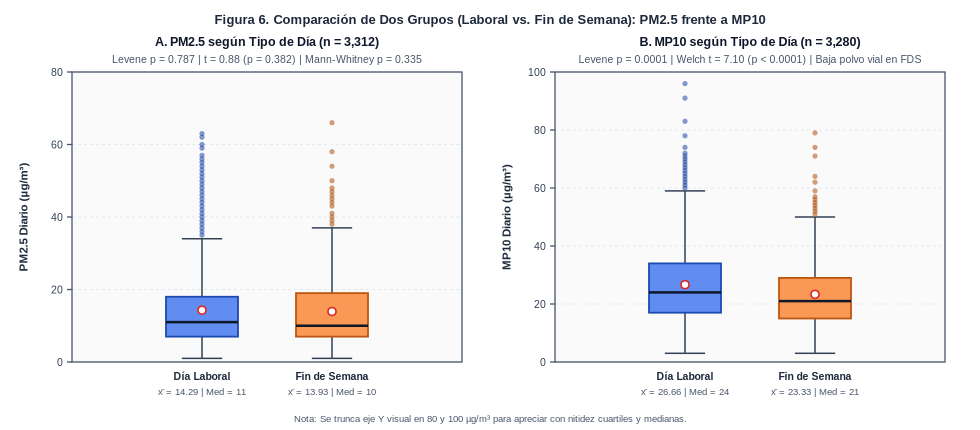
\includegraphics[width=\linewidth, height=0.43\textheight, keepaspectratio]{fig6_boxplot_dos_grupos_dia.png}
    \vspace{0.03cm}
    \begin{beamercolorbox}[wd=\linewidth, rounded=true, sep=2pt]{block body}
      \tiny\textbf{Contraste físico:} El $MP_{10}$ sí baja en fin de semana ($26.66 \to 23.33$, $t=7.10, p<0.0001$) por menor polvo vial, pero el \textbf{$PM_{2.5}$ permanece invariante} ($p=0.382$).
    \end{beamercolorbox}
  \end{column}

  \begin{column}{0.50\textwidth}
    \begin{alertblock}{\footnotesize Test 9 (Dos Grupos) — Hipótesis en Texto Natural}
      \scriptsize
      \begin{itemize}\setlength{\itemsep}{1pt}
        \item \textbf{$H_0$:} La concentración diaria media (y mediana poblacional) de $PM_{2.5}$ es idéntica durante los días laborales (Lun–Vie) y los fines de semana (Sáb–Dom).
        \item \textbf{$H_1$:} Existe una diferencia significativa en la concentración diaria de $PM_{2.5}$ entre días laborales y fines de semana por el cambio en actividad vehicular.
      \end{itemize}
    \end{alertblock}

    \begin{exampleblock}{\footnotesize Test 9 (Dos Grupos) — Hipótesis en Formato Matemático}
      \scriptsize
      \begin{itemize}\setlength{\itemsep}{1pt}
        \item \textbf{Paramétrico ($t$-Welch):} $H_0: \mu_{\text{Lab}} - \mu_{\text{FDS}} = 0 \;\;\text{vs.}\;\; H_1: \mu_{\text{Lab}} - \mu_{\text{FDS}} \neq 0$.\\
        Estadístico: $t = \frac{\bar{Y}_{\text{Lab}} - \bar{Y}_{\text{FDS}}}{\sqrt{s_1^2/n_1 + s_2^2/n_2}} = \frac{14.29 - 13.93}{0.41} = \mathbf{+0.88}$ ($v\text{-}p = \mathbf{0.382} > 0.10$).
        \item \textbf{No Paramétrico (Mann-Whitney):} $H_0: \text{Med}_{\text{Lab}} = \text{Med}_{\text{FDS}}$ ($11.0$ vs $10.0$, $p = \mathbf{0.335}$).
        \item \textbf{Decisión:} \textbf{No se rechaza $H_0$}. La calefacción a leña opera toda la semana sin descanso.
      \end{itemize}
    \end{exampleblock}
  \end{column}
\end{columns}
\end{frame}

% ==============================================================================
% DIAPOSITIVA 11: ETAPA 5.3B (4.1 PARTE 1) — ANOVA ESTACIONAL Y KRUSKAL-WALLIS
% ==============================================================================
\begin{frame}{4.1. Etapa 5.3B: ANOVA Estacional de 1 Factor y Kruskal-Wallis}
\framesubtitle{Tests N° 10 y 12: Descomposición $SCT = SC\text{Trat} + SCE$ y Magnitud de Efecto $\eta^2$}

\begin{columns}[T]
  \begin{column}{0.46\textwidth}
    \begin{block}{\footnotesize Tabla ANOVA de 1 Factor ($PM_{2.5}$ por Estación)}
      \renewcommand{\arraystretch}{1.0}
      \resizebox{\linewidth}{!}{
        \begin{tabular}{lrrrr}
          \toprule
          \textbf{Fuente (F.V.)} & \textbf{g.l.} & \textbf{Suma Cuad. ($SC$)} & \textbf{Media Cuad.} & \textbf{Test $F$} \\
          \midrule
          \textbf{Estación (Trat.)} & $3$ & $94.302,1$ & $31.434,0$ & $\mathbf{353.97}$ \\
          \textbf{Error (Dentro)} & $3308$ & $293.762,0$ & $88,8$ & ($p < 10^{-16}$) \\
          \midrule
          \textbf{Total} & $3311$ & $388.064,1$ & $\eta^2 = \mathbf{24.30\%}$ & \\
          \bottomrule
        \end{tabular}
      }
    \end{block}

    \begin{block}{\footnotesize Estadísticos por Nivel del Factor ($r=4$)}
      \renewcommand{\arraystretch}{0.95}
      \resizebox{\linewidth}{!}{
        \begin{tabular}{lrrrr}
          \toprule
          \textbf{Estación} & \textbf{$n_i$} & \textbf{Media $\bar{Y}_{i\cdot}$} & \textbf{Mediana} & \textbf{DE ($s_i$)} \\
          \midrule
          Verano & $760$ & $9.14$ & $8.00$ & $7.81$ \\
          Primavera & $832$ & $8.21$ & $8.00$ & $3.72$ \\
          \textbf{Otoño} & $828$ & $\mathbf{19.14}$ & $\mathbf{16.50}$ & $12.22$ \\
          \textbf{Invierno} & $892$ & $\mathbf{19.46}$ & $\mathbf{18.00}$ & $11.23$ \\
          \bottomrule
        \end{tabular}
      }
    \end{block}
  \end{column}

  \begin{column}{0.50\textwidth}
    \begin{alertblock}{\footnotesize Tests 10 y 12 (ANOVA y KW) — Texto Natural}
      \scriptsize
      \begin{itemize}\setlength{\itemsep}{1pt}
        \item \textbf{$H_0$:} La concentración diaria media (ANOVA) y mediana (Kruskal-Wallis) de $PM_{2.5}$ es igual en las cuatro estaciones del año (Verano, Otoño, Invierno y Primavera).
        \item \textbf{$H_1$:} Al menos una estación del año presenta una concentración media (o mediana) diaria de $PM_{2.5}$ significativamente distinta de las demás.
      \end{itemize}
    \end{alertblock}

    \begin{exampleblock}{\footnotesize Tests 10 y 12 (ANOVA y KW) — Formato Matemático}
      \scriptsize
      \begin{itemize}\setlength{\itemsep}{1pt}
        \item \textbf{Test 10 (ANOVA):} $H_0: \mu_{\text{Ver}} = \mu_{\text{Oto}} = \mu_{\text{Inv}} = \mu_{\text{Pri}} \;\;\text{vs.}\;\; H_1: \exists\,\mu_i \neq \mu_{i'}$.\\
        $F = \frac{MC\text{Trat}}{MCE} = \mathbf{353.97} > F_{0.05; 3, 3308} = 2.608$ ($p < 10^{-16}$). \textbf{Rechaza $H_0$}.
        \item \textbf{Test 12 (Kruskal-Wallis):} $H_0: \text{Med}_1=\dots=\text{Med}_4 \implies H(3) = \mathbf{942.29} > 7.815$ ($p < 10^{-16}$). \textbf{Rechaza $H_0$}. La estación explica el $\eta^2 = \mathbf{24.30\%}$ de la varianza.
      \end{itemize}
    \end{exampleblock}
  \end{column}
\end{columns}
\end{frame}

% ==============================================================================
% DIAPOSITIVA 12: ETAPA 5.3C (4.1 PARTE 2) — POST-HOC DE TUKEY HSD
% ==============================================================================
\begin{frame}{4.1 (Cont.). Etapa 5.3C: Procedimiento Post-Hoc de Tukey HSD}
\framesubtitle{Test N° 11: Comparaciones Múltiples por Pares de Estaciones (Tukey HSD)}

\begin{columns}[T]
  \begin{column}{0.46\textwidth}
    \centering
    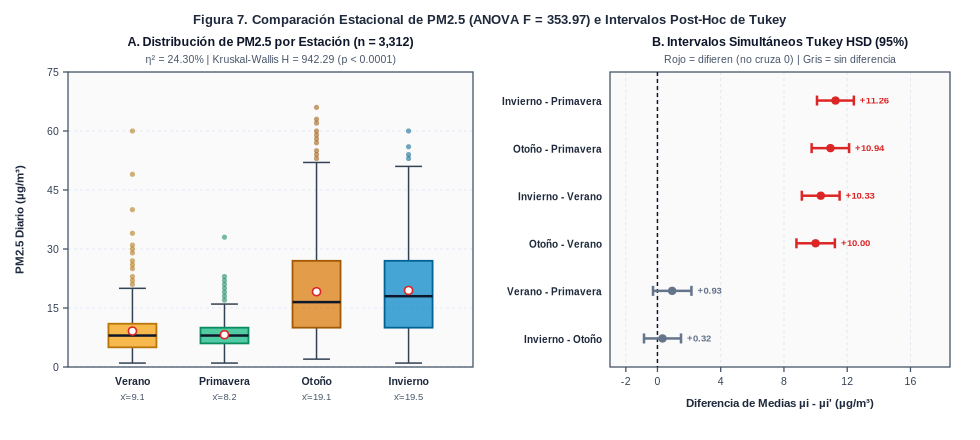
\includegraphics[width=\linewidth, height=0.45\textheight, keepaspectratio]{fig7_boxplot_tukey_estaciones.png}
    \vspace{0.02cm}
    {\tiny Izquierda: Boxplot estacional. Derecha: IC 95\% simultáneos de Tukey (Rojo = difieren; Gris = cruzan el 0).}
  \end{column}

  \begin{column}{0.50\textwidth}
    \begin{alertblock}{\footnotesize Test 11 (Tukey HSD) — Hipótesis en Texto Natural}
      \scriptsize
      \begin{itemize}\setlength{\itemsep}{1pt}
        \item \textbf{$H_0$:} Para cada par específico de estaciones $(i, i')$, sus medias poblacionales diarias de $PM_{2.5}$ son estadísticamente iguales entre sí.
        \item \textbf{$H_1$:} Las medias poblacionales del par de estaciones $(i, i')$ difieren significativamente entre sí.
      \end{itemize}
    \end{alertblock}

    \begin{exampleblock}{\footnotesize Test 11 (Tukey HSD) — Hipótesis en Formato Matemático}
      \scriptsize
      \begin{itemize}\setlength{\itemsep}{1pt}
        \item \textbf{Hipótesis:} $H_0: \mu_i - \mu_{i'} = 0 \;\;\text{vs.}\;\; H_1: \mu_i - \mu_{i'} \neq 0 \quad \forall i < i'$.
        \item \textbf{Estadístico y Criterio:} $T_{i,i'} = \frac{|\bar{Y}_{i\cdot} - \bar{Y}_{i'\cdot}|}{\sqrt{MCE/\tilde{n}_{i,i'}}} \ge q_{0.95; 4, 3308} = \mathbf{3.633}$ (o $0 \notin IC_{95\%}$).
        \item \textbf{Rechazan $H_0$ (4 pares inter-bloque):} Invierno y Otoño superan en $\mathbf{+10.0\text{ a }+11.26\,\mu\text{g/m}^3}$ a Verano y Primavera ($T \in [29.89, 35.05] > 3.633$).
        \item \textbf{No Rechazan $H_0$ (2 pares intra-bloque):} \textit{Otoño vs. Invierno} ($\Delta = 0.32, T = \mathbf{1.00}$) y \textit{Verano vs. Primavera} ($\Delta = 0.93, T = \mathbf{2.79}$) son iguales.
      \end{itemize}
    \end{exampleblock}
  \end{column}
\end{columns}
\end{frame}

% ==============================================================================
% DIAPOSITIVA 13: ETAPA 5.4 (4.2) — CATEGÓRICA VS CATEGÓRICA (CHI-CUADRADO)
% ==============================================================================
\begin{frame}{4.2. Etapa 5.4: Categórica vs. Categórica ($\chi^2$ y $V$ de Cramér)}
\framesubtitle{Test N° 13: Independencia entre Nivel Normativo de Alerta y Tipo de Día}

\begin{columns}[T]
  \begin{column}{0.46\textwidth}
    \centering
    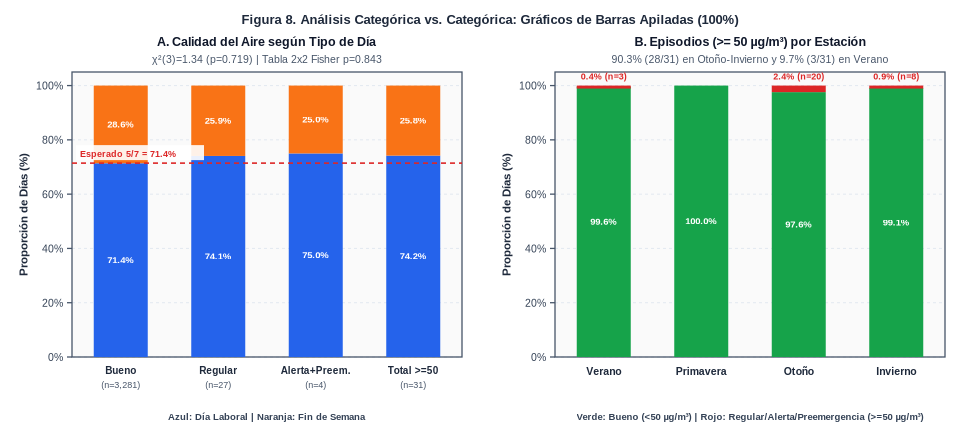
\includegraphics[width=\linewidth, height=0.39\textheight, keepaspectratio]{fig8_barras_apiladas_contingencia.png}
    \vspace{0.02cm}
    \renewcommand{\arraystretch}{0.92}
    \resizebox{\linewidth}{!}{
      \begin{tabular}{lrrrr}
        \toprule
        \textbf{Nivel Calidad} & \textbf{$O_{ij}$ Lab ($E_{ij}$)} & \textbf{$O_{ij}$ FDS ($E_{ij}$)} & \textbf{Total} & \textbf{\% Lab / FDS} \\
        \midrule
        Bueno ($<50$) & $2342$ ($2342.9$) & $939$ ($938.1$) & $3281$ & $71.4\% / 28.6\%$ \\
        Regular ($50\text{--}79$) & $20$ ($19.3$) & $7$ ($7.7$) & $27$ & $74.1\% / 25.9\%$ \\
        Alerta+Preem. ($\ge 80$) & $3$ ($2.9$) & $1$ ($1.1$) & $4$ & $75.0\% / 25.0\%$ \\
        \bottomrule
      \end{tabular}
    }
  \end{column}

  \begin{column}{0.50\textwidth}
    \begin{alertblock}{\footnotesize Test 13 (Independencia $\chi^2$) — Texto Natural}
      \scriptsize
      \begin{itemize}\setlength{\itemsep}{1pt}
        \item \textbf{$H_0$:} El nivel normativo diario de calidad del aire por $PM_{2.5}$ (Bueno, Regular, Alerta, Preemergencia) es estadísticamente independiente del tipo de día (Laboral vs. Fin de Semana).
        \item \textbf{$H_1$:} Existe dependencia estadística entre el nivel de alerta ambiental y el tipo de día de la semana.
      \end{itemize}
    \end{alertblock}

    \begin{exampleblock}{\footnotesize Test 13 (Independencia $\chi^2$) — Formato Matemático}
      \scriptsize
      \begin{itemize}\setlength{\itemsep}{1pt}
        \item \textbf{Hipótesis:} $H_0: P(A_i \cap D_j) = P(A_i)P(D_j) \;\;\forall (i,j) \quad \text{vs.} \quad H_1: P(A_i \cap D_j) \neq P(A_i)P(D_j)$.
        \item \textbf{Estadístico:} $\chi^2 = \sum_{i,j}\frac{(O_{ij}-E_{ij})^2}{E_{ij}} = \mathbf{1.3449} < \chi^2_{0.05, 3} = 7.815$ ($v\text{-}p = \mathbf{0.7185} > 0.10$).
        \item \textbf{Magnitud:} $V \text{ de Cramér} = \sqrt{\frac{\chi^2/n}{\min(r-1, k-1)}} = \mathbf{0.0202}$ (asociación nula).
        \item \textbf{Decisión:} \textbf{No se rechaza $H_0$}. Las alertas ocurren con igual probabilidad toda la semana.
      \end{itemize}
    \end{exampleblock}
  \end{column}
\end{columns}
\end{frame}

% ==============================================================================
% DIAPOSITIVA 14: SECCIÓN 6 (5.0) — ESPECIFICACIÓN DE 4 MODELOS Y ANOVA GLOBAL
% ==============================================================================
\begin{frame}{5. Modelamiento EMCO: Especificación de 4 Modelos y Test Global $F_c$}
\framesubtitle{Test N° 6: Significancia Global de la Regresión $\hat{\beta} = (X^T X)^{-1} X^T Y$}

\begin{columns}[T]
  \begin{column}{0.48\textwidth}
    \begin{block}{\footnotesize Especificación de los 4 Modelos ($n = 3.185$)}
      \scriptsize
      \begin{enumerate}\scriptsize\setlength{\itemsep}{2pt}
        \item \textbf{Modelo 1 (RLS Base, $p=1$):}
        $$PM_{2.5, i} = \beta_0 + \beta_1 MP_{10, i} + \epsilon_i$$
        \item \textbf{Modelo 2 (RLM + Gases, $p=4$):}
        $$PM_{2.5, i} = \beta_0 + \beta_1 MP_{10, i} + \beta_2 CO_i + \beta_3 NO_{2, i} + \beta_4 O_{3, i} + \epsilon_i$$
        \item \textbf{Modelo 3 (RLM + Gases + Dummies, $p=8$):}
        $$PM_{2.5, i} = \beta_0 + \beta_1 MP_{10} + \beta_2 CO + \beta_3 NO_2 + \beta_4 O_3 + \sum_{m=1}^3 \gamma_m D_m + \delta\text{FDS} + \epsilon_i$$
        \item \textbf{Modelo 4 (Log-Log Estacional, $p=4$):}
        $$\ln(PM_{2.5, i}) = \alpha_0 + \alpha_1 \ln(MP_{10, i}) + \alpha_2 \ln(CO_i) + \gamma_1 D_{\text{Oto}} + \gamma_2 D_{\text{Inv}} + u_i$$
      \end{enumerate}
    \end{block}
    {\tiny \textbf{Propiedades EMCO verificadas:} $\sum \hat{e}_i = 0$, $\sum Y_i = \sum \hat{Y}_i$, $X^T\hat{e} = 0$, $\hat{Y}^T\hat{e} = 0$, $SST = SSR + SSE$.}
  \end{column}

  \begin{column}{0.48\textwidth}
    \begin{alertblock}{\footnotesize Test 6 (ANOVA Regresión) — Texto Natural}
      \scriptsize
      \begin{itemize}\setlength{\itemsep}{1pt}
        \item \textbf{$H_0$:} Ninguna de las variables predictoras incluidas en el modelo tiene relación lineal con el $PM_{2.5}$; el modelo conjunto carece de capacidad explicativa.
        \item \textbf{$H_1$:} Al menos uno de los regresores incluidos contribuye significativamente a explicar y predecir la variación diaria de $PM_{2.5}$.
      \end{itemize}
    \end{alertblock}

    \begin{exampleblock}{\footnotesize Test 6 (ANOVA Regresión) — Formato Matemático}
      \scriptsize
      \begin{itemize}\setlength{\itemsep}{1.5pt}
        \item \textbf{Hipótesis:} $H_0: \beta_1 = \beta_2 = \dots = \beta_p = 0 \;\;\text{vs.}\;\; H_1: \exists\,\beta_j \neq 0$.
        \item \textbf{Estadístico:} $F_c = \frac{MSR}{MSE} = \frac{SSR/p}{SSE/(n-p-1)} \sim F_{(p, n-p-1)}$.
        \item \textbf{Resultados:} $M_1: F_c = \mathbf{6.927,0}$; $M_2: F_c = \mathbf{2.061,1}$; $M_3: F_c = \mathbf{1.924,6}$; $M_4: F_c = \mathbf{3.509,5}$ (todos con $v\text{-}p < 10^{-16}$).
        \item \textbf{Decisión:} \textbf{Se rechaza $H_0$} con evidencia muy fuerte en los 4 modelos.
      \end{itemize}
    \end{exampleblock}
  \end{column}
\end{columns}
\end{frame}

% ==============================================================================
% DIAPOSITIVA 15: SECCIÓN 6 (5.1 PARTE A) — TABLA COMPARATIVA Y CAMBIO F ANIDADO
% ==============================================================================
\begin{frame}{5.1 (Parte A): Comparación de Modelos y Prueba de Cambio $F$}
\framesubtitle{Test N° 8: Contraste de Cambio $F$ para Modelos Anidados ($M_1 \subset M_2 \subset M_3$)}

\begin{block}{\footnotesize Tabla Comparativa Multimétrica de los 4 Modelos ($n = 3.185$ días validados)}
  \renewcommand{\arraystretch}{0.96}
  \resizebox{\linewidth}{!}{
    \begin{tabular}{lrrrrrrrr}
      \toprule
      \textbf{Modelo Especificado} & \textbf{Regr. ($p$)} & \textbf{$R^2$ (\%)} & \textbf{$R_a^2$ Ajustado} & \textbf{Error Est. $S_e$} & \textbf{RMSE ($\mu\text{g/m}^3$)} & \textbf{MAE ($\mu\text{g/m}^3$)} & \textbf{Criterio AIC} & \textbf{Criterio BIC} \\
      \midrule
      \textbf{Modelo 1:} RLS Base ($MP_{10}$) & $1$ & $68.52\%$ & $68.51\%$ & $6.060$ & $6.058$ & $4.609$ & $11.478,7$ & $11.490,9$ \\
      \textbf{Modelo 2:} RLM + Gases ($CO, NO_2, O_3$) & $4$ & $72.16\%$ & $72.13\%$ & $5.701$ & $5.696$ & $4.359$ & $11.092,5$ & $11.122,8$ \\
      \textbf{Modelo 3:} RLM + Gases + Dummies Est./FDS & $8$ & $\mathbf{82.90\%}$ & $\mathbf{82.86\%}$ & $\mathbf{4.471}$ & $\mathbf{4.465}$ & $\mathbf{3.387}$ & $\mathbf{9.548,8}$ & $\mathbf{9.603,3}$ \\
      \textbf{Modelo 4:} Log-Log Estacional ($\ln PM_{2.5}$) & $4$ & $\mathbf{81.53\%}$ & $\mathbf{81.51\%}$ & $0.305^*$ & $\mathbf{3.860}^*$ & $\mathbf{2.715}^*$ & $-7.550,5^*$ & $-7.520,2^*$ \\
      \bottomrule
    \end{tabular}
  }
\end{block}

\vspace{0.04cm}
\begin{columns}[T]
  \begin{column}{0.48\textwidth}
    \begin{alertblock}{\footnotesize Test 8 (Cambio $F$ Anidado) — Texto Natural}
      \scriptsize
      \begin{itemize}\setlength{\itemsep}{1pt}
        \item \textbf{$H_0$:} Agregar el nuevo bloque de variables (gases en $M_2$ o dummies estacionales en $M_3$) no aporta reducción significativa del error residual respecto al modelo reducido.
        \item \textbf{$H_1$:} El bloque de nuevas variables reduce significativamente el error de predicción y mejora genuinamente el ajuste del modelo.
      \end{itemize}
    \end{alertblock}
  \end{column}

  \begin{column}{0.48\textwidth}
    \begin{exampleblock}{\footnotesize Test 8 (Cambio $F$ Anidado) — Formato Matemático}
      \scriptsize
      \begin{itemize}\setlength{\itemsep}{1pt}
        \item \textbf{Hipótesis:} $H_0: \beta_{q+1}=\dots=\beta_p=0 \;\;\text{vs.}\;\; H_1: \exists\,\beta_j \neq 0 \;\; (j > q)$.
        \item \textbf{Estadístico:} $F_{\text{cambio}} = \frac{(SSE_R - SSE_C)/(p-q)}{MSE_C} \sim F_{(p-q, n-p-1)}$.
        \item \textbf{Paso $M_1 \to M_2$:} $\Delta R^2 = +3.65\%$, $F(3, 3180) = \mathbf{138.92}$ ($p < 10^{-16}$). \textbf{Rechaza $H_0$}.
        \item \textbf{Paso $M_2 \to M_3$:} $\Delta R^2 = +10.74\%$, $F(4, 3176) = \mathbf{498.44}$ ($p < 10^{-16}$). \textbf{Rechaza $H_0$}.
      \end{itemize}
    \end{exampleblock}
  \end{column}
\end{columns}
\end{frame}

% ==============================================================================
% DIAPOSITIVA 16: SECCIÓN 6 (5.1 PARTE B) — VISUALIZACIÓN DE MODELOS EMCO
% ==============================================================================
\begin{frame}{5.1 (Parte B): Visualización del Ajuste y Efectos Estacionales}
\framesubtitle{Variación de pendiente por estación y valores Observados vs. Predichos ($Y$ vs. $\hat{Y}$)}

\begin{columns}[T]
  \begin{column}{0.52\textwidth}
    \centering
    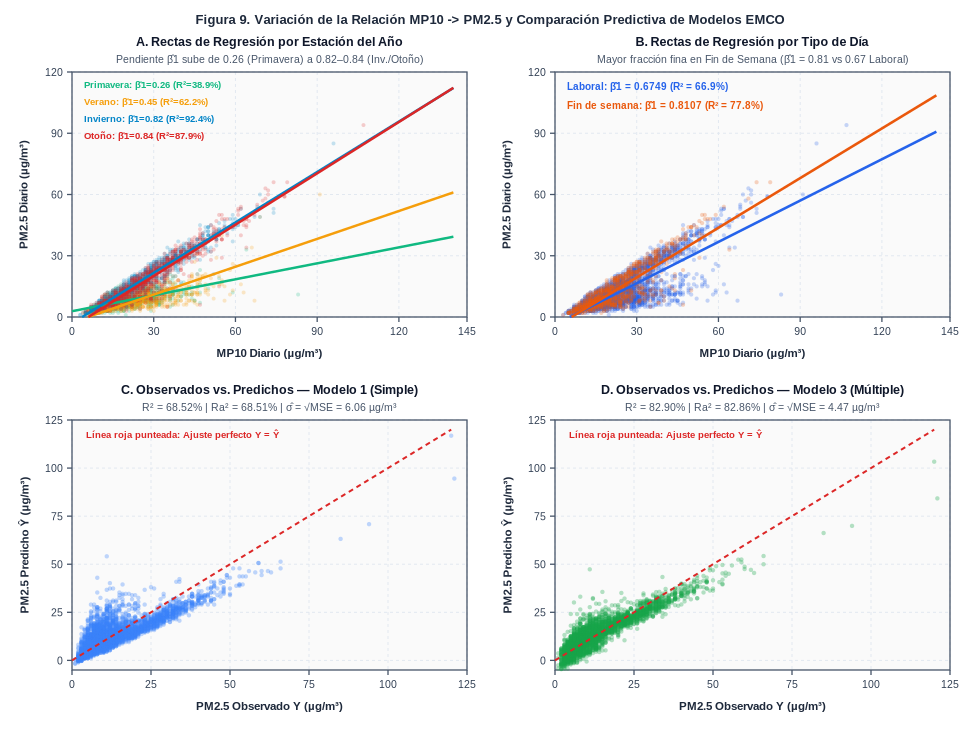
\includegraphics[width=\linewidth, height=0.62\textheight, keepaspectratio]{fig9_modelos_regresion_comparacion.png}
  \end{column}

  \begin{column}{0.44\textwidth}
    \begin{block}{\footnotesize Interpretación de los 4 Paneles (Fig. 9)}
      \scriptsize
      \begin{enumerate}\setlength{\itemsep}{3pt}
        \item \textbf{Cambio estructural de pendiente (Panel A):} En Primavera la fracción fina es baja ($\hat{\beta}_1 = 0.26$, polvo mineral/polen), mientras en \textbf{Invierno y Otoño sube a $\hat{\beta}_1 = 0.82\text{--}0.84$} ($R^2 \approx 90\%$) por humo de leña.
        \item \textbf{Efecto Fin de Semana (Panel B):} A igual nivel de $MP_{10}$, en fin de semana la pendiente es mayor ($0.81$ vs $0.67$) porque disminuye el polvo vial grueso pero persiste el humo fino domiciliario.
        \item \textbf{Reducción de dispersión (Paneles C vs. D):} Al pasar del Modelo 1 Simple ($R^2 = 68.52\%$) al \textbf{Modelo 3 Múltiple ($R^2 = 82.90\%$)}, la nube se ciñe estrechamente sobre la recta ideal $1:1$ ($Y = \hat{Y}$), bajando el AIC en $\mathbf{-1.930\text{ puntos}}$.
      \end{enumerate}
    \end{block}
  \end{column}
\end{columns}
\end{frame}

% ==============================================================================
% DIAPOSITIVA 17: SECCIÓN 6 (5.2) — INFERENCIA INDIVIDUAL BETA_J, IC 95% Y VIF
% ==============================================================================
\begin{frame}{5.2. Inferencia Individual ($\beta_j$), IC 95\% y Multicolinealidad (VIF)}
\framesubtitle{Test N° 7: Contraste $t$ de Significancia Individual Parcial}

\begin{columns}[T]
  \begin{column}{0.50\textwidth}
    \begin{block}{\footnotesize Coeficientes EMCO Modelo 3 ($R^2 = 82.90\%$)}
      \renewcommand{\arraystretch}{0.95}
      \resizebox{\linewidth}{!}{
        \begin{tabular}{lrrrrl}
          \toprule
          \textbf{Regresor $X_j$} & \textbf{Coef. $\hat{\beta}_j$} & \textbf{Estad. $t_c$} & \textbf{Valor-$p$} & \textbf{IC 95\% $[\text{LI}, \text{LS}]$} & \textbf{VIF} \\
          \midrule
          Intercepto (Ver.) & $-7.929$ & $-25.49$ & $< 10^{-16}$ & $[-8.538, -7.319]$ & — \\
          \textbf{$MP_{10}$} & $\mathbf{+0.620}$ & $\mathbf{+79.64}$ & $< 10^{-16}$ & $[+0.605, +0.636]$ & $\mathbf{1.59}$ \\
          \textbf{$CO$ (ppm)} & $\mathbf{+4.748}$ & $\mathbf{+14.32}$ & $< 10^{-16}$ & $[+4.098, +5.398]$ & $\mathbf{1.70}$ \\
          $NO_2$ (ppb) & $-0.076$ & $-2.50$ & $0.0125$ & $[-0.136, -0.016]$ & $2.14$ \\
          $O_3$ (ppb) & $-0.094$ & $-5.43$ & $< 0.0001$ & $[-0.128, -0.060]$ & $1.16$ \\
          \textbf{$D_{\text{Otoño}}$} & $\mathbf{+7.396}$ & $\mathbf{+31.47}$ & $< 10^{-16}$ & $[+6.935, +7.857]$ & $1.66$ \\
          \textbf{$D_{\text{Invierno}}$} & $\mathbf{+8.827}$ & $\mathbf{+37.33}$ & $< 10^{-16}$ & $[+8.363, +9.291]$ & $1.75$ \\
          $D_{\text{Primavera}}$ & $+2.161$ & $+9.19$ & $< 10^{-16}$ & $[+1.700, +2.622]$ & $1.66$ \\
          $\text{Es\_FDS}$ & $+1.779$ & $+9.95$ & $< 10^{-16}$ & $[+1.428, +2.129]$ & $\mathbf{1.04}$ \\
          \bottomrule
        \end{tabular}
      }
    \end{block}
    {\tiny \textbf{En Modelo 2 (sin dummies):} $NO_2$ ($p=0.423$) y $O_3$ ($p=0.573$) incluyen al $0$ en su IC 95\% (\textbf{No rechazan $H_0$}).}
  \end{column}

  \begin{column}{0.46\textwidth}
    \begin{alertblock}{\footnotesize Test 7 ($t$ Individual) — Texto Natural}
      \scriptsize
      \begin{itemize}\setlength{\itemsep}{1pt}
        \item \textbf{$H_0$:} Manteniendo constantes las demás variables (\textit{ceteris paribus}), el predictor $X_j$ no tiene efecto lineal parcial sobre el $PM_{2.5}$.
        \item \textbf{$H_1$:} El predictor $X_j$ aporta un efecto parcial significativo sobre el $PM_{2.5}$.
      \end{itemize}
    \end{alertblock}

    \begin{exampleblock}{\footnotesize Test 7 ($t$ Individual) — Formato Matemático}
      \scriptsize
      \begin{itemize}\setlength{\itemsep}{1pt}
        \item \textbf{Hipótesis:} $H_0: \beta_j = 0 \;\;\text{vs.}\;\; H_1: \beta_j \neq 0 \quad \Big|\quad t_c = \frac{\hat{\beta}_j}{se(\hat{\beta}_j)} \sim t_{(n-p-1)}$.
        \item \textbf{Criterio:} Rechazar $H_0$ si $|t_c| > 1.9607$ (equivalente a $0 \notin IC_{95\%}$).
        \item \textbf{Hallazgos:} \textbf{Rechazan $H_0$} $MP_{10}$ ($t_c=79.6$), $CO$ ($t_c=14.3$) y el salto invernal ($\mathbf{+8.83\,\mu\text{g/m}^3}$). Todos los $\text{VIF} \le 2.14 \ll 5$ (sin multicolinealidad).
      \end{itemize}
    \end{exampleblock}
  \end{column}
\end{columns}
\end{frame}

% ==============================================================================
% DIAPOSITIVA 18: SECCIÓN 6 (5.3 PARTE A) — SUPUESTOS Y PRUEBAS SOBRE RESIDUOS
% ==============================================================================
\begin{frame}{5.3 (Parte A): Diagnóstico Formal de los 6 Supuestos del EMCO}
\framesubtitle{Contrastes de Homocedasticidad (Breusch-Pagan) y Autocorrelación (Durbin-Watson)}

\begin{columns}[T]
  \begin{column}{0.48\textwidth}
    \begin{block}{\footnotesize Auditoría de los 6 Supuestos}
      \scriptsize
      \begin{enumerate}\setlength{\itemsep}{1.5pt}
        \item \textbf{S1 Linealidad y S3 ($E[\epsilon|X]=0$):} Cumplido ($\sum \hat{e}_i = 0$).
        \item \textbf{S2 Rango Completo y VIF:} Cumplido ($\text{VIF}_{\max} = 2.14 < 5.0$).
        \item \textbf{S4a Homocedasticidad (Breusch-Pagan):} El Modelo 4 Log-Log reduce el estadístico $LM$ en un $\mathbf{-86\%}$ ($690.9 \to 124.8$).
        \item \textbf{S4b Autocorrelación (Durbin-Watson):} $d = 0.735$ ($\rho_1 = 0.63$), reflejando persistencia meteorológica multidiaria.
        \item \textbf{S6 Normalidad Residual e Influencia:} En Modelo 3, asimetría $k_s = \mathbf{-0.36} \in [-0.5, 0.5]$ ($W = 0.968$). Por TLC ($n=3.185$), inferencia válida. Distancia de Cook $\max D_i = \mathbf{0.118 \ll 1.0}$ (sin distorsión).
      \end{enumerate}
    \end{block}
  \end{column}

  \begin{column}{0.48\textwidth}
    \begin{alertblock}{\footnotesize Tests de Breusch-Pagan y DW — Texto Natural}
      \scriptsize
      \begin{itemize}\setlength{\itemsep}{1pt}
        \item \textbf{Breusch-Pagan:} $H_0$: La varianza del error es constante en todo nivel de contaminación (homocedasticidad) vs. $H_1$: La dispersión del error crece en episodios altos (heterocedasticidad).
        \item \textbf{Durbin-Watson:} $H_0$: Los errores diarios son independientes en el tiempo vs. $H_1$: Existe persistencia serial entre días seguidos.
      \end{itemize}
    \end{alertblock}

    \begin{exampleblock}{\footnotesize Tests de Breusch-Pagan y DW — Formato Matemático}
      \scriptsize
      \begin{itemize}\setlength{\itemsep}{1pt}
        \item \textbf{Breusch-Pagan:} $H_0: \text{Var}(\epsilon_i|X_i) = \sigma^2 \;\;\text{vs.}\;\; H_1: \text{Var}(\epsilon_i|X_i) = h(X_i\alpha)$.\\
        $LM = n\cdot R^2_{\hat{e}^2} \sim \chi^2_{(p)} \implies$ Cae de $690.9$ (M3) a $\mathbf{124.8}$ en M4 Log-Log.
        \item \textbf{Durbin-Watson:} $H_0: \rho_1 = 0 \;\;\text{vs.}\;\; H_1: \rho_1 > 0 \quad \Big|\quad d = \frac{\sum(\hat{e}_t - \hat{e}_{t-1})^2}{\sum \hat{e}_t^2} = \mathbf{0.735}$.
      \end{itemize}
    \end{exampleblock}
  \end{column}
\end{columns}
\end{frame}

% ==============================================================================
% DIAPOSITIVA 19: SECCIÓN 6 (5.3 PARTE B) — PANEL GRÁFICO DE RESIDUOS EMCO
% ==============================================================================
\begin{frame}{5.3 (Parte B): Verificación Gráfica en los Residuos del EMCO}
\framesubtitle{Comportamiento de Residuos en Modelo 3 Lineal vs. Estabilización en Modelo 4 Log-Log}

\begin{columns}[T]
  \begin{column}{0.52\textwidth}
    \centering
    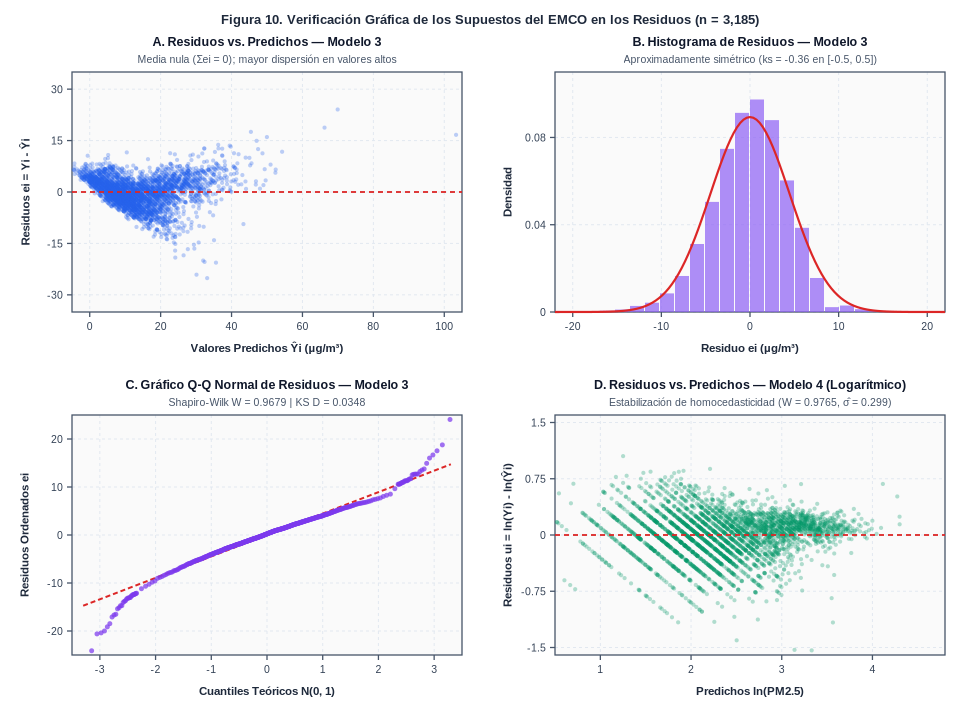
\includegraphics[width=\linewidth, height=0.62\textheight, keepaspectratio]{fig10_diagnostico_residuos_emco.png}
  \end{column}

  \begin{column}{0.44\textwidth}
    \begin{block}{\footnotesize Lectura Diagnóstica de los 4 Paneles (Fig. 10)}
      \scriptsize
      \begin{itemize}\setlength{\itemsep}{3pt}
        \item \textbf{Panel A (Residuos vs. Predichos M3):} Media exactamente nula ($\sum \hat{e}_i = 0$) sin curvatura parabólica, validando linealidad. Se aprecia la apertura en abanico durante episodios críticos invernales.
        \item \textbf{Paneles B y C (Histograma y Q-Q Normal M3):} Al incluir gases y dummies, los residuos alcanzan simetría ($k_s = -0.36$, dentro del rango $[-0.5, 0.5]$ de clases) con ajuste Gaussiano central ($W = 0.9679$).
        \item \textbf{Panel D (Residuos Modelo 4 Log-Log):} La transformación logarítmica elimina el efecto cono y estabiliza la banda horizontal de varianza ($\hat{\sigma} = 0.299$, $W = 0.9765$), logrando el menor error predictivo ($\text{RMSE} = \mathbf{3.86\,\mu\text{g/m}^3}$).
      \end{itemize}
    \end{block}
  \end{column}
\end{columns}
\end{frame}

% ==============================================================================
% DIAPOSITIVA 20: CUADRO MAESTRO OFICIAL DE LAS 13 HIPÓTESIS DEL ESTUDIO
% ==============================================================================
\begin{frame}{6. Cuadro Maestro Oficial de las 13 Hipótesis del Estudio}
\framesubtitle{Síntesis Obligatoria en Formato Texto Natural y Formato Matemático ($\alpha = 0.05$)}

\renewcommand{\arraystretch}{0.96}
\resizebox{\linewidth}{!}{
  \begin{tabular}{clllll}
    \toprule
    \textbf{N°} & \textbf{Prueba / Test} & \textbf{Hipótesis en Texto Natural ($H_0$ vs. $H_1$)} & \textbf{Hipótesis Matemática} & \textbf{Estadístico / Criterio} & \textbf{Decisión ($\alpha=0.05$)} \\
    \midrule
    \textbf{1} & \textbf{Test de Grubbs} (Etapa 4) & $H_0$: Sin atípicos extremos vs. $H_1$: Al menos un atípico real. & $H_0$: No outliers vs. $H_1: \exists X_i$ extremo & $G = \mathbf{9.87} > G_{\text{crit}} = 4.30$ & \textbf{Rechaza $H_0$} ($p<.001$) \\
    \textbf{2} & \textbf{Kolmogórov-Smirnov} (5.1) & $H_0$: Distribución Normal en centro vs. $H_1$: No es Normal. & $H_0: F_X = \Phi$ vs. $H_1: F_X \neq \Phi$ & $D = \mathbf{0.1644} > 0.0236$ & \textbf{Rechaza $H_0$} ($p<.001$) \\
    \textbf{3} & \textbf{Anderson-Darling} (5.1) & $H_0$: Ajuste Normal en colas vs. $H_1$: Colas pesadas no normales. & $H_0: X \sim \mathcal{N}$ vs. $H_1: X \nsim \mathcal{N}$ (colas) & $A^{2*} = \mathbf{151.16} \gg 0.787$ & \textbf{Rechaza $H_0$} ($\ln: 8.47$) \\
    \textbf{4} & \textbf{Pearson ($r$)} (Etapa 5.2) & $H_0$: Sin relación lineal vs. $H_1$: Asociación lineal positiva. & $H_0: \rho = 0$ vs. $H_1: \rho > 0$ & $r = \mathbf{0.8293}, t_c = \mathbf{84.98}$ & \textbf{Rechaza $H_0$} ($p<10^{-16}$) \\
    \textbf{5} & \textbf{Spearman ($r_s$)} (Etapa 5.2) & $H_0$: Sin correlación monótona vs. $H_1$: Dependencia monótona $+$. & $H_0: \rho_s = 0$ vs. $H_1: \rho_s > 0$ & $r_s = \mathbf{0.7771}, z_s = \mathbf{44.49}$ & \textbf{Rechaza $H_0$} ($p<10^{-16}$) \\
    \textbf{6} & \textbf{ANOVA Regresión ($F_c$)} & $H_0$: Modelo lineal no explica $PM_{2.5}$ vs. $H_1$: Modelo es predictivo. & $H_0: \beta_1=\dots=\beta_p=0$ vs. $H_1: \exists \beta_j \neq 0$ & $F_c = \mathbf{1.924,6} > F_{0.05}$ & \textbf{Rechaza $H_0$} ($p<10^{-16}$) \\
    \textbf{7} & \textbf{Test $t$ Individual ($\beta_j$)} & $H_0$: Regresor $X_j$ no aporta (\textit{ceteris paribus}) vs. $H_1$: Efecto real. & $H_0: \beta_j = 0$ vs. $H_1: \beta_j \neq 0$ & $|t_c| > 1.96$ ($0 \notin IC_{95\%}$) & \textbf{Rechaza:} $MP_{10}, CO$, Estac. \\
    \textbf{8} & \textbf{Cambio $F$ Anidado} (Sec. 6) & $H_0$: Nuevos bloques no mejoran vs. $H_1$: Reducción real de error. & $H_0: \beta_{\text{bloque}} = 0$ vs. $H_1: \Delta SSE > 0$ & $F_{\text{cambio}} = \mathbf{498.44} > F_{0.05}$ & \textbf{Rechaza $H_0$} ($p<10^{-16}$) \\
    \textbf{9} & \textbf{t-Welch / Mann-Whitney} & $H_0$: Igual $PM_{2.5}$ en laboral y FDS vs. $H_1$: Difieren por tráfico. & $H_0: \mu_{\text{Lab}} = \mu_{\text{FDS}}$ ($\text{Med}_1=\text{Med}_2$) & $t = \mathbf{0.88}, v\text{-}p = \mathbf{0.382}$ & \textbf{No Rechaza $H_0$} ($v\text{-}p>0.10$) \\
    \textbf{10} & \textbf{ANOVA 1 Factor} (5.3) & $H_0$: Igual media en 4 estaciones vs. $H_1$: Difieren por estación. & $H_0: \mu_{\text{Ver}}=\mu_{\text{Oto}}=\mu_{\text{Inv}}=\mu_{\text{Pri}}$ & $F = \mathbf{353.97} > 2.61$ & \textbf{Rechaza $H_0$} ($\eta^2 = 24.3\%$) \\
    \textbf{11} & \textbf{Post-Hoc Tukey HSD} & $H_0$: Par $(i,i')$ tiene igual media vs. $H_1$: Medias del par difieren. & $H_0: \mu_i - \mu_{i'} = 0$ vs. $H_1: \mu_i \neq \mu_{i'}$ & $T_{i,i'} \ge 3.633$ ($0 \notin IC$) & \textbf{Rechaza:} Inv/Oto vs Ver/Pri \\
    \textbf{12} & \textbf{Kruskal-Wallis ($H$)} (5.3) & $H_0$: Igual mediana estacional vs. $H_1$: Dominancia invernal. & $H_0: \text{Med}_1=\dots=\text{Med}_4$ & $H(3) = \mathbf{942.29} > 7.82$ & \textbf{Rechaza $H_0$} ($p<10^{-16}$) \\
    \textbf{13} & \textbf{Chi-cuadrado ($\chi^2$)} (5.4) & $H_0$: Nivel Alerta independiente de Tipo de Día vs. $H_1$: Asociados. & $H_0: P(A_i \cap D_j) = P(A_i)P(D_j)$ & $\chi^2 = \mathbf{1.345}, p = \mathbf{0.719}$ & \textbf{No Rechaza $H_0$} ($V = 0.02$) \\
    \bottomrule
  \end{tabular}
}

\vspace{0.06cm}
\begin{beamercolorbox}[wd=\textwidth, rounded=true, sep=2.5pt]{block body example}
  \tiny\textbf{Síntesis Inferencial:} Los 13 contrastes convergen: el $PM_{2.5}$ está gobernado por el $MP_{10}$ ($\hat{\beta}_1 \approx 0.62\text{--}0.70$), el trazador de leña $CO$ ($t_c=14.3$) y el invierno ($\Delta \approx +8.8\,\mu\text{g/m}^3$), siendo \textbf{invariante al día laboral}.
\end{beamercolorbox}
\end{frame}

% ==============================================================================
% DIAPOSITIVA 21: DISCUSIÓN, LIMITACIONES E IMPLICANCIAS PRÁCTICAS (35%)
% ==============================================================================
\begin{frame}{7. Discusión, Limitaciones e Implicancias Prácticas (35\%)}
\framesubtitle{Conexión con literatura científica y políticas públicas (PPDA Gran Concepción)}

\begin{columns}[T]
  \begin{column}{0.48\textwidth}
    \begin{block}{\footnotesize Respuestas a la Pregunta de Investigación}
      \scriptsize
      \begin{enumerate}\scriptsize\setlength{\itemsep}{2pt}
        \item \textbf{Capacidad predictiva superior ($R^2 = 82.90\%$):} Integrar $CO$ y estacionalidad eleva el ajuste del $68.5\%$ al $82.9\%$, reduciendo el RMSE a $4.47\,\mu\text{g/m}^3$ (y hasta $\mathbf{3.86\,\mu\text{g/m}^3}$ en Modelo 4 Log-Log).
        \item \textbf{Rol trazador del $CO$ ($t_c = 14.32$):} Discrimina si un día de alto $MP_{10}$ proviene de polvo mineral (primavera/verano, $\hat{\beta}_1 = 0.26$) o humo de biomasa (invierno, $\hat{\beta}_1 = 0.82\text{--}0.84$), validando a \textit{Cereceda-Balic et al. (2020)}.
        \item \textbf{Invarianza al día de la semana:} El $PM_{2.5}$ no baja en fin de semana ($p = 0.382$ y $\chi^2\,p = 0.719$), confirmando a \textit{Gramsch et al. (2021)} y \textit{Saide et al. (2016)}.
      \end{enumerate}
    \end{block}
  \end{column}

  \begin{column}{0.48\textwidth}
    \begin{alertblock}{\footnotesize Limitaciones Metodológicas}
      \scriptsize
      \begin{itemize}\scriptsize\setlength{\itemsep}{1pt}
        \item \textbf{Variables omitidas:} Sin viento ni altura de capa límite en SINCA; capturadas vía dummies y $O_3$.
        \item \textbf{Inercia serial ($DW = 0.735$):} Eventos invernales duran 2–4 días; extensión futura: rezagos $SARIMAX$ o errores HAC.
      \end{itemize}
    \end{alertblock}

    \begin{exampleblock}{\footnotesize Implicancias Prácticas (PPDA D.S. N° 6/2019)}
      \scriptsize
      \begin{itemize}\scriptsize\setlength{\itemsep}{1pt}
        \item \textbf{Imputación operativa:} Los Modelos 3 y 4 reconstruyen fallas del monitor fino con $R^2 > 82\%$.
        \item \textbf{Política pública:} Como las alertas persisten el fin de semana, el foco debe ser el \textbf{recambio de calefactores a leña y aislación térmica}, no restricciones vehiculares laborales.
      \end{itemize}
    \end{exampleblock}
  \end{column}
\end{columns}

\vspace{0.10cm}
\centering
{\footnotesize\bfseries\color{UddNavy} ¡Muchas gracias por su atención! Quedamos atentos a sus preguntas y comentarios.}
\end{frame}

\end{document}
